\documentclass[border=12pt]{article} 
\usepackage[dvipsnames]{xcolor}
\usepackage{tikz}
\usepackage[lining]{libertine}
\usepackage[]{xcolor}
\usepackage{fourier}
% see https://www.unk.edu/ccr/marketing-advertising/branding-and-identity-marks/files/UNK-graphics-standards-quick-guide.pdf

\definecolor{UNKblue}{HTML}{002F6C}
\definecolor{UNKgold}{HTML}{CC8A00}
\newenvironment{tightcenter}{%
  \setlength\topsep{-20pt}
  \setlength\parskip{-10pt}
  \begin{center}
}{%
  \end{center}
}

\usetikzlibrary{shadows}
\begin{document}
\LARGE
  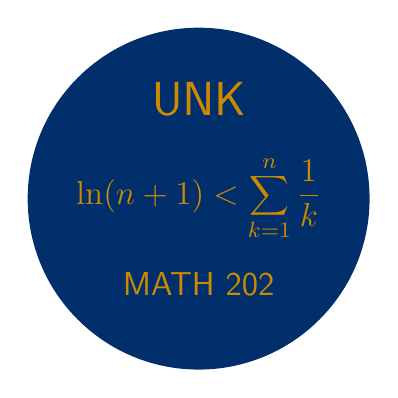
\begin{tikzpicture}
    \node[circle,minimum width=1.5in,text=UNKgold,fill=UNKblue,font=\sffamily] at (0,0) {  
      \begin{minipage}[c]{1.25in}  
        \vspace{-0.1in}
      \begin{tightcenter}  \LARGE UNK  \end {tightcenter} \hfill   \\ 
        \vspace{0.05in}
        \large \begin{tightcenter}  
            \(\displaystyle \ln(n+1) < \sum_{k=1}^n \frac{1}{k} \)  \end{tightcenter}  \hfill  \\ 
      \vspace{0.15in}
            \large \begin{tightcenter} MATH 202   \end{tightcenter} \end{minipage} };
  \end{tikzpicture}


\end{document}
